
Flow cytometry (FCM) data are multivariate measurements from flow cytometers that record light scatter and fluorescence emission properties of hundreds of thousands of individual cells. They are important to studying the cell structures of normal and abnormal cells and diagnosing human disease \cite{cytometry_nature}. This is a challenging dataset for clustering because the distribution of the data is non-Gaussian and heavily skewed.

We experimented on DLBCL dataset from the FlowCAP challenge \cite{cytometry_nature}. It contains 30 samples, and each sample consists of tens of thousands of cells measurements in 5 dimensions, with 2 to 4 clusters. Each sample is a separate clustering task, and the performance is evaluated by the weighted f-score used in \cite{cytometry_nature}. We split the 5 dimensions into three views, 1 and 2 as the first view, 3 and 4 the second and 5 the last view. For each sample, we selected the best kernel bandwidth by log-likelihood with 5-fold cross validation. For comparison, we also evaluated the performance of EM algorithm for mixture of Gaussians (GMM) with diagonal covariances with 20 restarts. Figure~\ref{fig:real_data} presents the results sorted by sample size. Our method (kernel spectral) outperforms GMM on samples where the three views are conditionally independent because it can adapt well to highly skew distributions. However, in a few samples, some views are strongly correlated, resulting in degraded performance. \bxcomment{The poor performance on some samples makes it difficult to discuss the results.}


\begin{figure*}
  \centering
  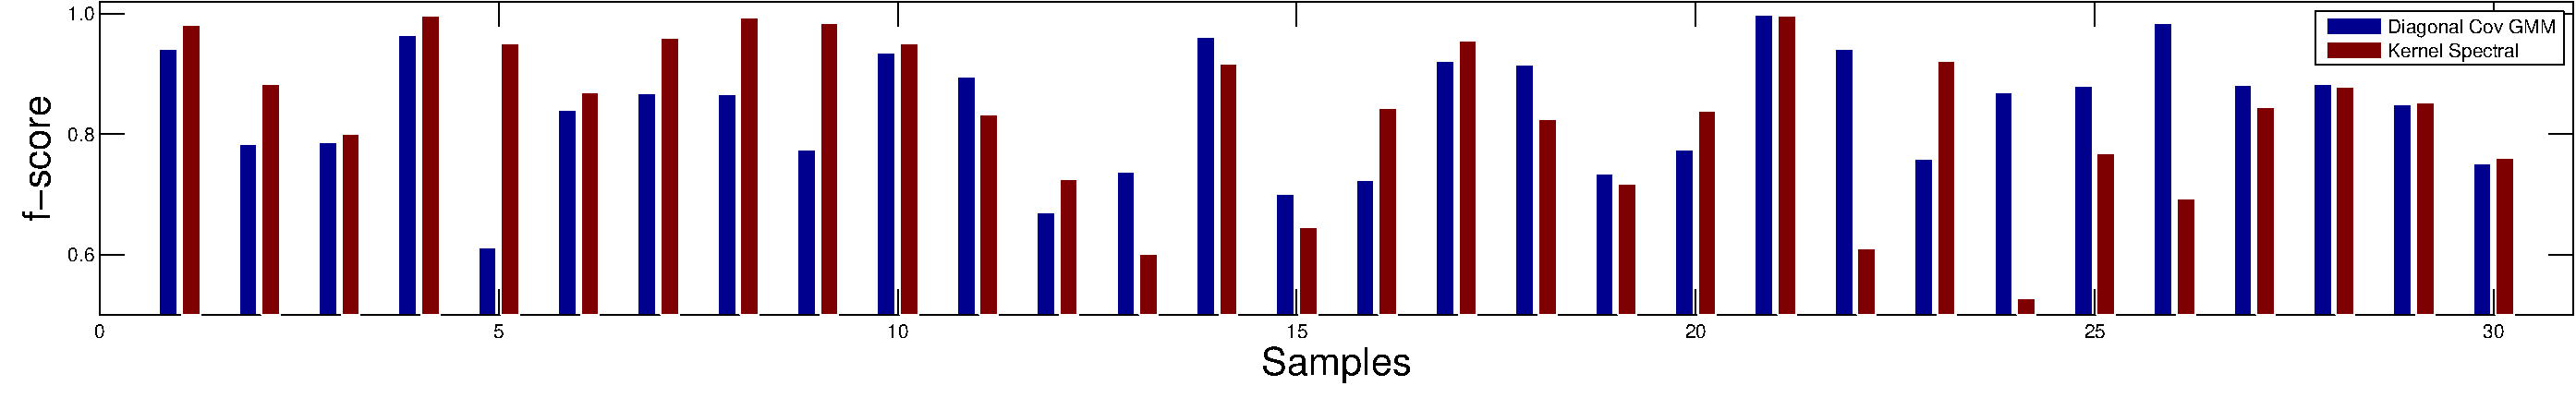
\includegraphics[width=0.9\textwidth]{../experiment/figure/paired_bar_chat} 
   \vspace{-3mm}
  \caption{Clustering results on DLBCL flow cytometry data. There are 30 samples, and each group of bars represents f-scores from mixture of Gaussian with diagonal covariances and kernel spectral method. The samples are ordered by increasing sample size.}\label{fig:real_data}
  \vspace{-3mm}
\end{figure*}
